%!TEX root = ../dissertation.tex
\chapter{Definitions}\label{ch:definitions}
\newthought{We present definitions and explanations} of concepts and terms that are used throughout this work.

\section{Rules}
A \textit{rule} is an IF-THEN statement consisting of a boolean antecedent and a classification label.
We are working in the realm of binary classification, so the label is either a 0 or a 1.
The boolean antecedents are generated from the rule mining mechanism and are a conjunction of boolean features.
These antecedents are satisfied by some data points (also called \textit{samples}) and not for others.
We say a rule \textit{classifies} a given data point when the antecedent is satisfied for that data point.
As we combine these rules into rule lists, only the first rule that classifies any given data point can make a prediction for that data point.
Thus, we say a rule \textit{captures} a given data point if it is the first rule in a rule list to classify that data point.

\section{Rule Lists}
%Let us define a training dataset of size N as $\{x_n, y_n\}_{n=1}^N$ where each $x_n \in \{0, 1\}^J$ are binary features and each $y_n \in \{0, 1\}$ are binary labels.
%Each rule $x_n$ therefore classifies some of the data points (those indices where $x_{n, j} = 1$).
%Define a rulelist $\mathbf{r} = (r_1, r_2, ... , r_k, r_0)$ where each $r_i \in \{x_n\}_{n=1}^N, \forall i > 0$.
%$r_0$ is defined as the default rule, which makes a prediction on all data points that are not captured in rules $1 ... k$. 
A \textit{rule list} is an ordered collection of rules.
As defined above, rules have an inherent accuracy based on what data they classify and how they predict the label.
When they are placed into a rule list, however, their accuracy is based on what data they capture---which is usually not the same as what data they classify.
They can perform better or worse than their inherent accuracy depending on what rules come before them in a given rule list.
Thus, our algorithm is focused on finding the list composed of the best rules and the order that maximizes predictive accuracy.
A rule list also has a \textit{default rule}, placed at the end of all of these rules, that classifies all data points and predicts the majority label.
This allows a rule list to make predictions for all points because any point not captured by the pre-mined rules is therefore captured by the default rule.
We refer to the set of rules that compose a rule list, not including the default rule, as a \textit{prefix}.

\begin{figure}[t!]
%\vspace{-3mm}
\begin{algorithmic}
\normalsize
\State \bif $(age=23-25) \wedge (priors=2-3)$ \bthen $yes$
\State \belif $(age=18-20)$ \bthen $yes$
\State \belif $(sex=male) \wedge (age=21-22)$ \bthen $yes$
\State \belif $(priors>3)$ \bthen $yes$
\State \belse $no$
\end{algorithmic}
%\vspace{-3mm}
\caption{An example rule list that predicts two-year recidivism for the COMPAS dataset, found by CORELS.}
\label{fig:rule-list}
\end{figure}

\section{Objective Function}
Rule lists have a loss function based on the number of points that are misclassified by the rules in the rule list.
We define our \textit{objective} function to be the sum of that loss and a regularization term.
We use a \textit{regularization} term, which is a constant times the length of the rule list.
This has the effect of preventing overfitting on training data sets as well as preventing extremely long, and therefore uninterpretable, rule lists.
While the objective is related to accuracy (a higher accuracy means a lower objective), we will be optimizing over the objective function instead of just the accuracy in order to get the benefits of the regularization term.

\begin{math}
objective(RL) = loss(RL) + c * len(RL)
\end{math}

\section{Bounds}\label{sec:bounds}
For a set of $n$ rules, there are $n!$ possible rule lists.
Finding the optimal rule list using a brutal force is infeasible for any problem of reasonable size.
Our algorithm uses the discrete optimization technique of branch-and-bound to solve the combinatorially difficult problem of finding an optimal rule list.
This requires tight bounds that allow us to prune as much of the search space as possible.
These bounds are formalized and proved in Angelino et al. \cite{AngelinoLaAlSeRu17} and are reproduced in Appendix A.
For clarity we present informal summaries of the important bounds here.

\subsection{Lower Bound}
We use the term \textit{lower bound} to mean the best possible outcome for the objective function for a given prefix.
We do this by calculating the error of the prefix and assuming that any points uncaptured by the prefix will be predicted correctly.
This is equivalent to assuming that the default rule captures all points perfectly.
Because any future extensions of the prefix can only ever make mistakes, we will be able to use it to prune our exploration.
An important property of the lower bound is that it increases monotonically.

\subsection{Hierarchical Objective Bound}
The main bound for our algorithm is the \textit{hierarchical objective bound}. 
It says that we do not need to purse a rule list if it has a lower bound that is worse than the best objective we have already seen.
This follows from the fact that lower bounds increase monotonically, so if the lower bound of rule list A is worse than the objective of rule list B, any extensions of rule list A can never be better than rule list B.
This allows us to prune large parts of the search space by not pursuing rule lists that could never be better than something we've already seen.

\begin{figure}
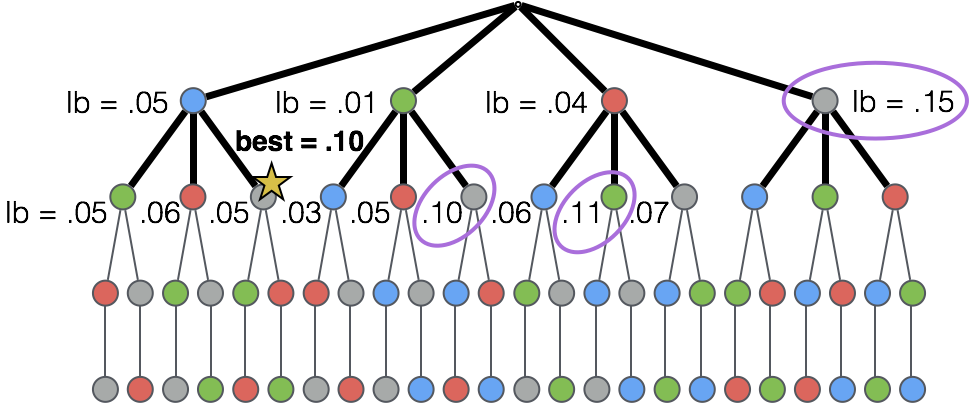
\includegraphics[width=0.5\textwidth]{figs/ela_branch-and-bound-tree.png}
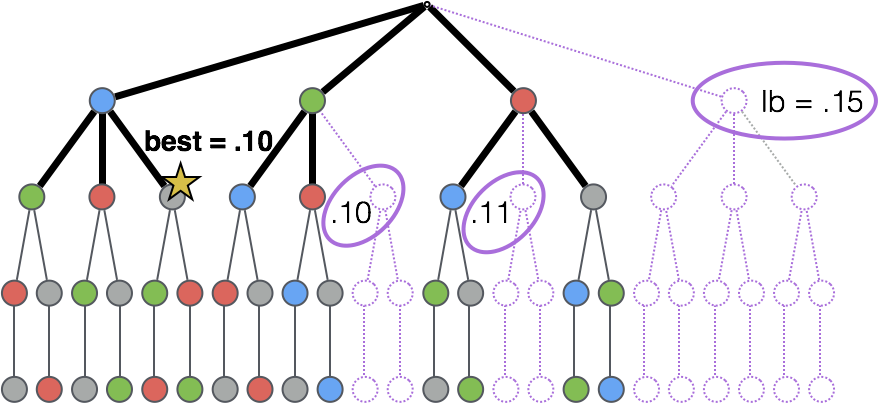
\includegraphics[width=0.5\textwidth]{figs/ela_branch-and-bound-tree-pruned.png}
\caption[Objective bound]{This tree shows the hierarchical objective bound in action. Our best objective seen is the prefix (blue, gray) with an objective of $0.10$. Any prefixes with lower bound greater than this objective--(gray), (red, green), (green, gray) can be pruned and not ever looked at.
\label{fig:objective-bound}}
\end{figure}

\subsection{Permutation Bound}

As defined above, every sample is captured by precisely one rule--any sample that is caught by rule A in the rule list AB cannot be caught by rule B. 
Now consider a \textit{permutation} of the rule list AB: the rule list BA.
Any samples that are captured by either rule A or B but not both will be captured identically in both rule lists.
Samples that are captured by both rules will again be captured the same in both rule lists, though they may be predicted differently in the two rule lists.
Thus, regardless of the order in which the rules appear, rule lists AB and BA will capture exactly the same set of data.
They will differ only in which rules capture which samples, so their accuracy may differ. 
We can use this knowledge to create a bound as follows.
If we know that the lower bound of AB is better than the lower bound of BA, we can eliminate from consideration all rule lists beginning with BA.
This is due to the fact that any corresponding rule list beginning with AB will capture exactly the same samples as the equivalent rule list beginning with BA but will have a better objective score.
We can eliminate all but one permutation of a given set of rules using this principle.

\begin{figure}
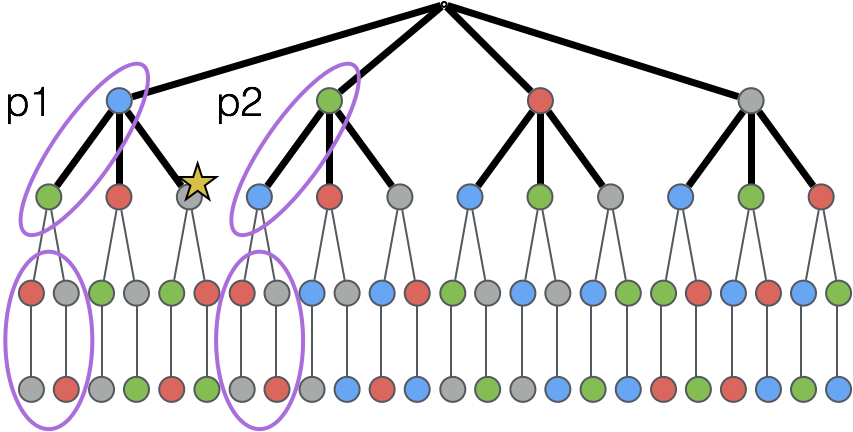
\includegraphics[width=0.5\textwidth]{figs/ela_branch-and-bound-permutations.png}
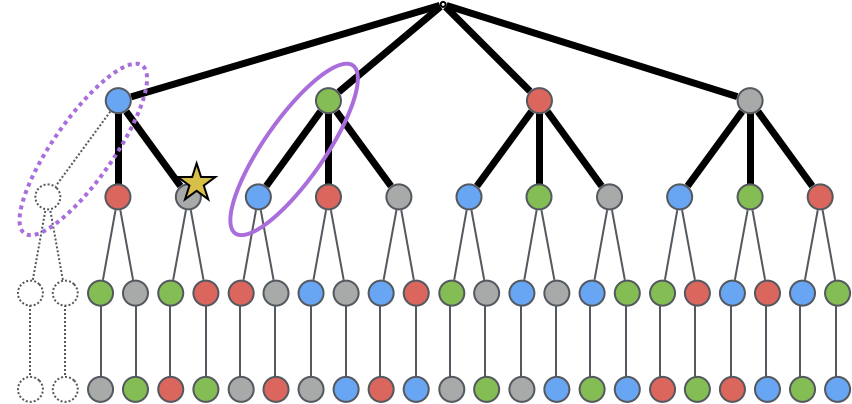
\includegraphics[width=0.5\textwidth]{figs/ela_branch-and-bound-permutations-pruned.png}
\caption[Permutation bound]{This tree shows the use of the permutation bound. Prefixes (blue, green) and (green, blue) are permutations of each other, so their lower bounds can be compared. The prefix (green, blue) has a better lower bound, so (blue, green) can be pruned and none of its children have to be examined.
\label{fig:permutation-bound}}
\end{figure}

\subsection{Support Bounds}
Due to our regularization term in calculating our objective function, adding a rule that does little to help our accuracy will actually be harmful to the overall objective score.
This allows us to place bounds that rely on the \textit{support} of the rules we add.
It never makes sense to add a rule that increases the objective function, so we only consider adding rules that capture enough points correctly to overcome the regularization penalty.
By definition, rules that don't capture enough of the remaining points cannot capture them correctly, so this provides us with two closely related bounds.
As our rule lists get longer many rules do not capture enough points that haven't already been captured and this bound begins to play an even larger role.

\subsection{Equivalent Points Bound}
This bound relies on the structure of our dataset.
In our dataset, we may encounter two data points that have the same features but different labels.
We call the set of these data points \textit{equivalence points}, and describe the label that occurs less often as the \textit{minority} label.
Any rule that classifies one point in an equivalence class will also classify all other points in that class.
However, it is impossible to correctly predict equivalence points with different labels using a single rule.
So, for a given class of equivalence points, we know that we will mispredict all of the points with a minority label.
We can thus update our lower bound to be tighter than just assuming that the default rule will capture all remaining points correctly.
Now, we assume all remaining points will be captured incorrectly if it is an equivalent point with a minority label.
This gives us much tighter lower bounds and in practice allows us to prune much more efficiently.

\section{Curiosity}
There are a number of different ways to explore the search space (see \ref{sec:queue}).
Some methods, such as BFS, prioritize exploration---looking at all rule lists of a given length before proceeding to the next length.
Others, such as a priority queue ordered by lower bound, focus on purely exploiting the best prefixes that we've seen.
We define a new metric, \textit{curiosity}, that blends together both exploration and exploitation.
Curiosity is a function of both the lower bound and the number of samples captured.
This prioritizes rule lists that still have many samples left to capture (exploration) while also pursuing rule lists with promising lower bounds (exploitation).

\begin{math}
curiosity(RL) = lowerBound(RL) - c * (len(RL) - 1)  * (nsamples / |captured(RL)|)
\end{math}

\section{Remaining Search Space}
One metric for tracking the efficacy of our optimizations will be seeing how quickly we reduce the remaining search space.
We start with a combinatorially large search space, but quickly prune it down using our bounds.
We calculate the remaining search space is by looking at all of the potential prefixes in our  queue and seeing how much each prefix could potentially be expanded.
Due to our regularization term, we are able to bound the maximum length of a prefix as our best objective gets updated.
This upper bound on the maximum length of a viable prefix allows us to place an upper bound on the search space as well.
We find that the remaining search space decreases rapidly at the beginning of execution, then slowly decreases until the very end of execution when it again rapidly decreases.